\documentclass{article}

\def\sectionnumber{4.5}
\def\sectiontitle{Midterm Review}

\usepackage{midterm}
\usepackage{graphicx} %package to manage images
\graphicspath{ {./images/} }

% Set this false to hide, true to show
\setboolean{showanswers}{true}

\begin{document}

\header

\vspace{10mm}

1. (a) Let $X\sim$ Pois$(\lambda)$. Find $E(e^X)$ (simplify).

\hide{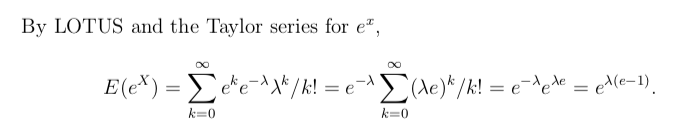
\includegraphics[scale=0.5]{images/midterm1a.png}}

1. (b) The numbers $1,2,3,...,n$ are listed in some random order (with all $n!$ permutations equally likely).  An inversion occurs each time a pair of numbers is out of order, i.e., the larger number is earlier in the list than the smaller number.  For example, $3,1,4,2$ has 3 inversions (3 before 1, 3 before 2, 4 before 2).  Find the expected number of inversions in the list (simplify).

\hide{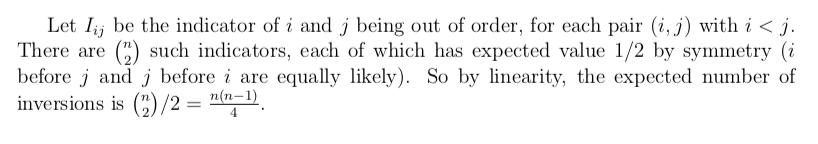
\includegraphics[scale=0.5]{images/midterm1b.png}}

\newpage

2. A group of 360 people are going to be split into 120 teams of 3 (where the order of teams and the order within a team don’t matter).

(a) How many ways are there to do this (simplified, in terms of factorials)?

\hide{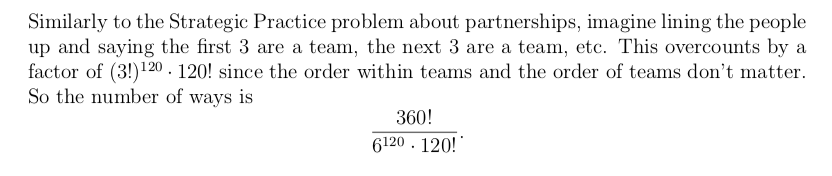
\includegraphics[scale=0.5]{images/midterm2a.png}}

(b) The  360  people  consist  of  180  married  couples.   A  random  split  into  teams  of  3 is  chosen,  with  all  possible  splits  equally  likely.   Find  the  expected  number  of  teams containing married couples.  (You can leave your answer in terms of binomial coefficients and  a  product  of  a  few  terms,  but  you  should  not  have  summations  or  complicated expressions in your final answer.)

\hide{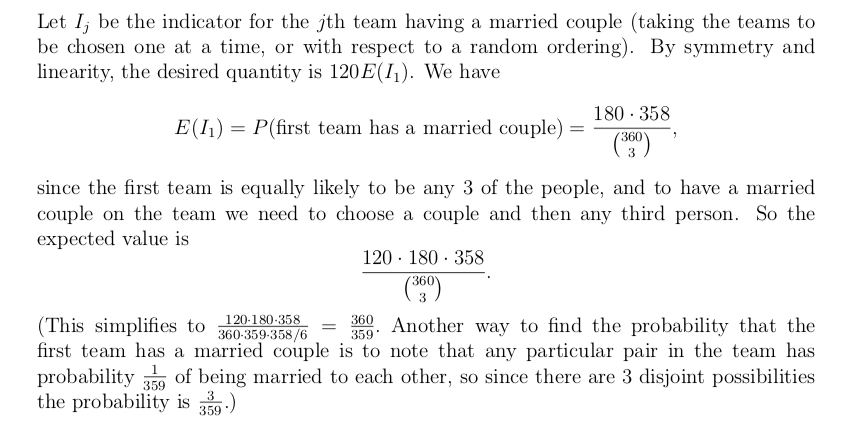
\includegraphics[scale=0.5]{images/midterm2b.png}}

\newpage

3. A certain college has $g$ good courses and $b$ bad courses, where $g$ and $b$ are positive integers.  Alice, who is hoping to find a good course, randomly shops courses one at a time (without replacement) until she finds a good course.

(a) Find  the  expected  number  of  bad  courses  that  Alice  shops  before  finding  a  good course (as a simple expression in terms of $g$ and $b$).

\hide{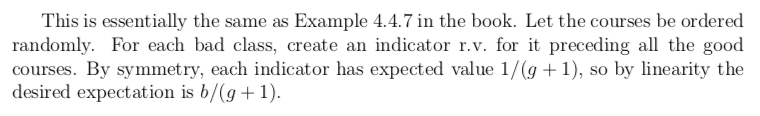
\includegraphics[scale=0.5]{images/midterm3a.png}}

(b) Should the answer to (a) be less than, equal to, or greater than $b/g$?  Explain this using properties of the Geometric distribution.

\hide{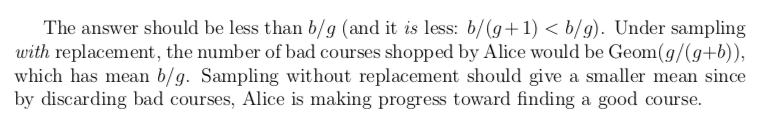
\includegraphics[scale=0.5]{images/midterm3b.png}}

\newpage

4. A certain baby cries if and only if she is hungry, tired, or both.  Let $C$ be the event that the baby is crying, $H$ be the event that she is hungry, and $T$ be the event that she is tired.  Let $P(C) =c$, $P(H) =h$, and $P(T) =t$, where none of $c$, $h$, $t$ are equal to 0 or 1.  Suppose that $H$ and $T$ are independent.

(a) Find $c$, in terms of $h$ and $t$. (Simplify fully.)

\hide{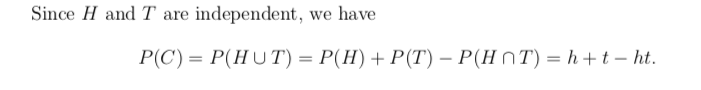
\includegraphics[scale=0.5]{images/midterm4a.png}}

(b) Find $P(H|C)$, $P(T|C)$, and $P(H,T|C)$ (in terms of $c$,$h$,$t$; simplify fully).

\hide{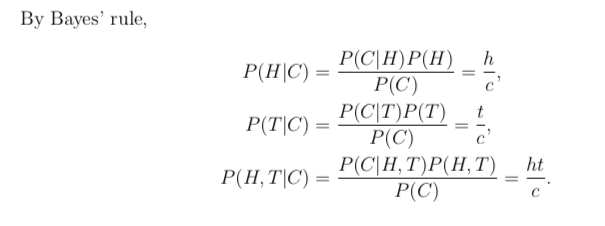
\includegraphics[scale=0.5]{images/midterm4b.png}}

(c) Are $H$ and $T$ conditionally independent given $C$?  Justify your answer in two ways: algebraically using the quantities from (b), and with a brief but clear intuitive explanation in words.

\hide{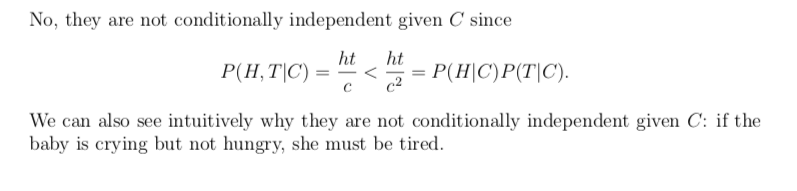
\includegraphics[scale=0.5]{images/midterm4c.png}}

\newpage

5. A new treatment for a disease is being tested, to see whether it is better than the standard treatment.  The existing treatment is effective on 50\% of patients.  It is believed initially that there is a 2/3 chance that the new treatment is effective on 60\% of patients,and a 1/3 chance that the new treatment is effective on 50\% of patients.  In a pilot study,the new treatment is given to 20 random patients, and is effective for 15 of them.

(a) Given  this  information,  what  is  the  probability  that  the  new  treatment  is  better than the standard treatment (as an unsimplified number)?

\hide{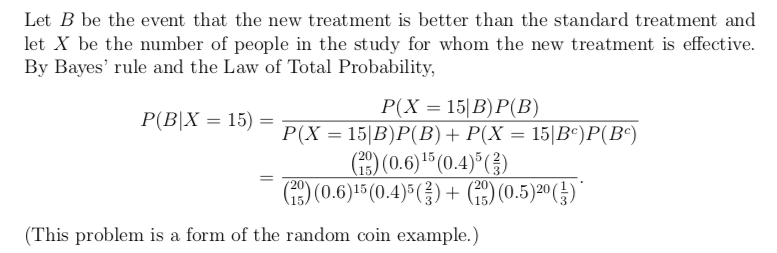
\includegraphics[scale=0.5]{images/midterm5a.png}}

(b) A second study is done later, giving the new treatment to 20 new random patients. Given the results of the first study, what is the PMF for how many of the new patients the new treatment is effective on?  (Don’t simplify; letting $p$ be the answer to (a), your answer can be left in terms of $p$.)

\hide{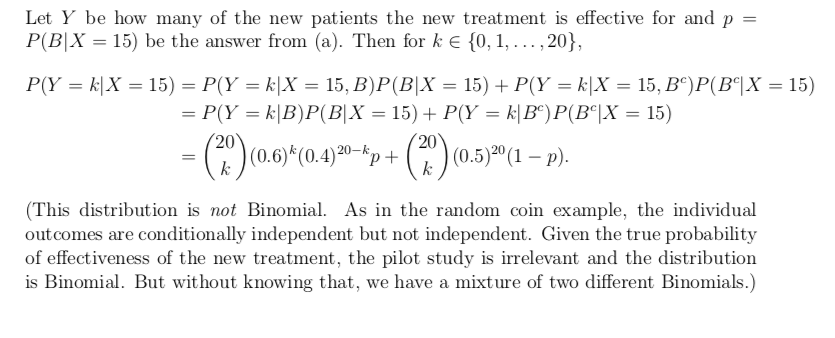
\includegraphics[scale=0.5]{images/midterm5b.png}}

\end{document}